
\documentclass[final]{beamer}



\usepackage[scale=0.8,size=a1]{beamerposter} % Use the beamerposter package for laying out the poster

\usetheme{confposter} % Use the confposter theme supplied with this template
\usepackage{multicol}
\setbeamercolor{block title}{fg=dblue,bg=white} % Colors of the block titles
\setbeamercolor{block body}{fg=black,bg=white} % Colors of the body of blocks
\setbeamercolor{block alerted title}{fg=white,bg=dblue!70} % Colors of the highlighted block titles
\setbeamercolor{block alerted body}{fg=black,bg=dblue!10} % Colors of the body of highlighted blocks
% Many more colors are available for use in beamerthemeconfposter.sty

%-----------------------------------------------------------
% Define the column widths and overall poster size
% To set effective sepwid, onecolwid and twocolwid values, first choose how many columns you want and how much separation you want between columns
% In this template, the separation width chosen is 0.024 of the paper width and a 4-column layout
% onecolwid should therefore be (1-(# of columns+1)*sepwid)/# of columns e.g. (1-(4+1)*0.024)/4 = 0.22
% Set twocolwid to be (2*onecolwid)+sepwid = 0.464
% Set threecolwid to be (3*onecolwid)+2*sepwid = 0.708

\newlength{\sepwid}
\newlength{\onecolwid}
\newlength{\twocolwid}
\newlength{\threecolwid}
\setlength{\paperwidth}{33.1in} % A0 width: 46.8in
\setlength{\paperheight}{23.4in} % A0 height: 33.1in
\setlength{\sepwid}{0.0\paperwidth} % Separation width (white space) between columns
\setlength{\onecolwid}{0.22\paperwidth} % Width of one column
\setlength{\twocolwid}{0.464\paperwidth} % Width of two columns
\setlength{\threecolwid}{0.708\paperwidth} % Width of three columns
\setlength{\topmargin}{-0.5in} % Reduce the top margin size
%-----------------------------------------------------------

\usepackage{graphicx}  % Required for including images

\usepackage{booktabs} % Top and bottom rules for tables
\usepackage{standalone} % to load standalone file (itkz picture for ex)
\usepackage{array} %finest gestion of tabular

%----------------------------------------------------------------------------------------
%	TITLE SECTION 
%----------------------------------------------------------------------------------------

%\title{Exploring the dynamic of cultural changes: A model to understand the amphorae production patterns in the Roman Empire} % Poster title
\title{New perspective on the study of variations in Amphorae production during the Roman Empire} % Poster title

\author{Maria Coto, Simon Carrignon and Xavier Rubio-Campillo} % Author(s)

\institute{Barcelona Supercomputing Center - University of Barcelona} % Institution(s)

%----------------------------------------------------------------------------------------

\begin{document}

\addtobeamertemplate{block end}{}{\vspace*{2ex}} % White space under blocks
\addtobeamertemplate{block alerted end}{}{\vspace*{2ex}} % White space under highlighted (alert) blocks

\setlength{\belowcaptionskip}{2ex} % White space under figures
\setlength\belowdisplayshortskip{2ex} % White space under equations

\begin{frame}[t] % The whole poster is enclosed in one beamer frame

\begin{columns}[t] % The whole poster consists of three major columns, the second of which is split into two columns twice - the [t] option aligns each column's content to the top

\begin{column}{\sepwid}\end{column} % Empty spacer column

\begin{column}{\onecolwid} % The first column


\begin{block}{Introduction}

\justify

Material culture variability allows us to understand the interpretation of the change processes. In particular, we want to identify changes on the amphorae production and if making techniques processes were related with the spatial distribution. We think that amphorae made in nearby workshops should share more similar traits than amphorae made from farthest workshops. As hypothesis, production techniques would be vertically transmitted based on the learning from master to disciple instead of horizontal transmission where this learning is done by workers with the same level. Empirical studies and theoretical model were propose to test this hypothesis.
 
  
\end{block}


\begin{block}{Dataset}

\justify
We analysed 413 amphorae (Dressel 20, \emph{cf} Fig~\ref{fig:betica}~(b)) from 4 different workshops located in \emph{Baetica} \textbf{(fig.\ref{fig:betica}~(a))}. Amphorae production in this province was really important and active during 300 years in the Roman Empire. The workshops were selected from different sites of \emph{Baetica} province in order to know if morphometric distance was correlated with spatial distance. A set 90 samples from each workshop were used to create a database. 8 measures focused on the rim were taken from each amphorae sample. 

\begin{figure}
\begin{tabular}{cc}


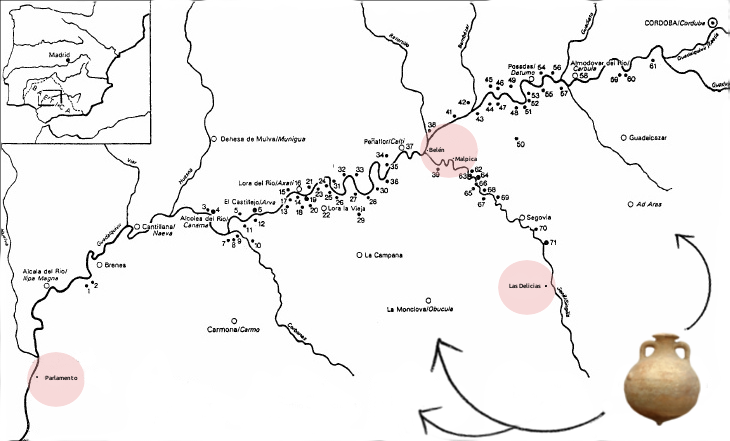
\includegraphics[width=0.7\linewidth]{images/fig1.png} &
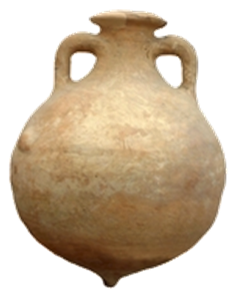
\includegraphics[width=0.2\linewidth]{images/amphorae.png} \\
(a) & (b)
\end{tabular}

\caption{a) More than 80 pottery workshops were distributed along rivers Guadalquivir and Genil. Red circles belong to the workshops analysed. b) Dressel 20 amphora}
\label{fig:betica}
\end{figure}


 \end{block}
\end{column} % End of the first column

%BEGIN THE SECOND COLUMN-------------------------------------------------
\begin{column}{\twocolwid}


\begin{block}{Exploration of empirical data}
\begin{columns}[t,totalwidth=\twocolwid]



\begin{column}{\onecolwid} %first subcolumn left


{\textbf{Principal Component Analysis}} 
\justify

PCA was used to explore these metrical observations with the 8 measurement as variables. Results allow us to simplify the analysis by grouping the variance of the dataset. The first two principal components were chosen to see the significant differences among workshops. 

\vspace{1cm}
{\textbf{Results}}\\
\justify
Figure~\ref{fig:pca} suggests that amphorae from closer workshops tend to be more similar. Most of the workshop have different signals on PC1 (i.e. Bel\'en, Delicias and Malpica) while Parlamento shows a distinctive pattern on PC2.


\end{column}

\begin{column}{\sepwid}\end{column} % Empty spacer column

\begin{column}{\onecolwid} %first subcolumn right


\begin{figure}
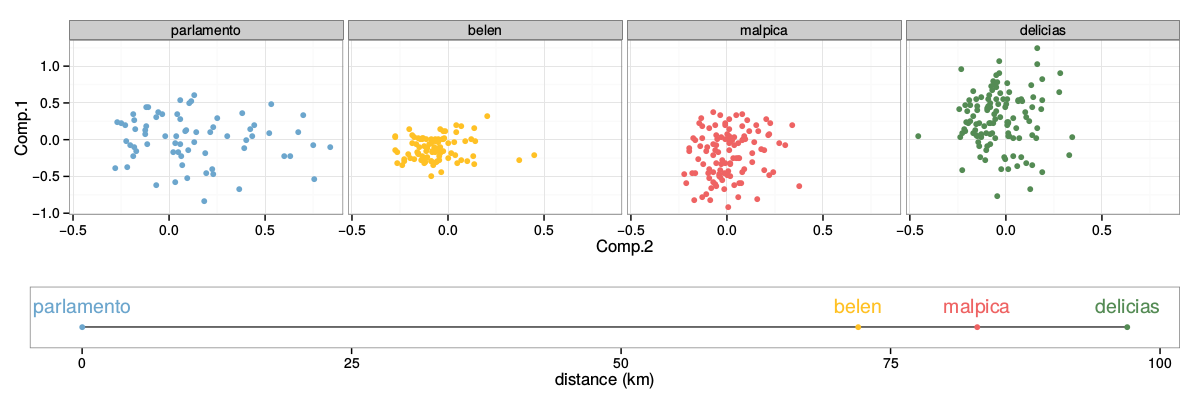
\includegraphics[width=0.6\linewidth]{images/fig2.png}
\caption{First and Second Principal Components First for amphorae measured from 4 different workshops}
\label{fig:pca}
\end{figure}

\end{column}
 % End of the second column
\end{columns}

\end{block}

\begin{block}{Theoretical Exploration}

\begin{columns}[t,totalwidth=\twocolwid]

\begin{column}{1.025\onecolwid} %first subcolumn left
%on the left

{\textbf{Model}}\\
\justify
We propose a simple model where a fixed number of workshop produce a fixed amount of amphora during a certain time following a certain techniques. Every 100 time step each workshop have a certain probability to slightly modify their production technique or to copy the one used by another workshop. 
\begin{figure}
	    \centering
	%\resizebox{}{!}{
    \documentclass{standalone}

\begin{document}
    \begin{tikzpicture}[thick,scale=2]
		\coordinate (WS0) at (0,0);
		\coordinate (WS1) at (1,0);
		\coordinate (WS2) at (2,0);
		\coordinate (WS3) at (3,0);
		\draw[thick,-] (0,0) -- (3,0) node[anchor=north west] {};   
		\foreach \x in {0,1,2,3}
		\draw (\x cm,2pt) -- (\x cm,-2pt) node[anchor=north] {$WS_\x$};


		\draw [black,shorten <= 0.25cm, shorten >= 0.25cm, <->] (WS1) to[out=80,in=100,distance=1cm] node[above,font=\scriptsize]{knowledge transmission} (WS3); 


	\draw [black,shorten <= 0.7cm, shorten >= 0.7cm, <->] (WS0) to[out=-80,in=-100,distance=.75cm	]  node[font=\scriptsize,pos=.60	,above]{$T_{0 \rightarrow 1}$} (WS1);
	\draw [black,shorten <= 0.7cm, shorten >= 0.7cm, <->] (WS0) to[out=-80,in=-100,distance=1cm	]  node[font=\scriptsize,pos=.75	,above]{$T_{0 \rightarrow 2}$}(WS2);
	\draw [black,shorten <= 0.7cm, shorten >= 0.7cm, <->] (WS0) to[out=-80,in=-100,distance=1.25cm	]  node[font=\scriptsize,pos=.82		,above]{$T_{0 \rightarrow 3}$}(WS3);

    \end{tikzpicture}

\end{document}


%}
    \caption{Schema of the model}
    \label{fig:mod}
\end{figure}

{\textbf{Horizontal Transmission}}\\
\justify
To test the impact of horizontal transmission on the variation in production between the workshop, we introduce a penalties: workshop more farer to $WS_0$ has lesser chance to make a cultural copy ($p=f(d)$ with $d$ the distance to $WS_0$)


\end{column}

%\begin{column}{.2\sepwid}\end{column} % Empty spacer column

\begin{column}{1.025\onecolwid} %first subcolumn right
\justify

{\textbf{Result}}\\
\justify
If the probability of horizontal transfer of knowledge between workshop is high the variation between the production is low. If the probability of cultural transfer is low, the variability is high, till it reaches its maximum where no horizontal transfer is allowed.

    \begin{figure}[h!]
    \centering
	\caption{Evolution of the variation of the mean of the observed measure between the workshops for different Horizontal Transmission penalities}
	%\begin{tabular}{m{.3\textwidth}m{.3\textwidth}m{.3\textwidth}}
    \begin{tabular}{ccc}
	     $f(d)=d$ & $f(d)=d^3$ & No Copy\\
	    
	    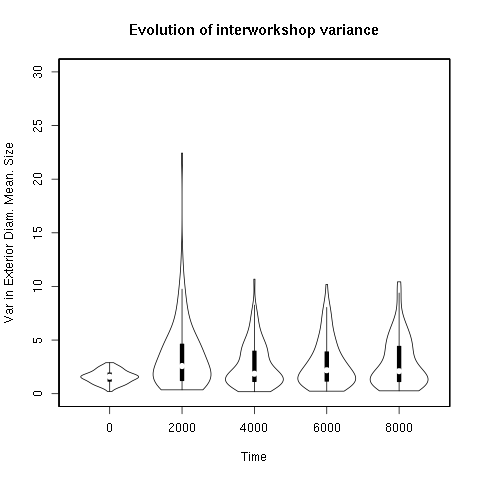
\includegraphics[height=.3\textwidth]{images/lineC.png}
	    &
	    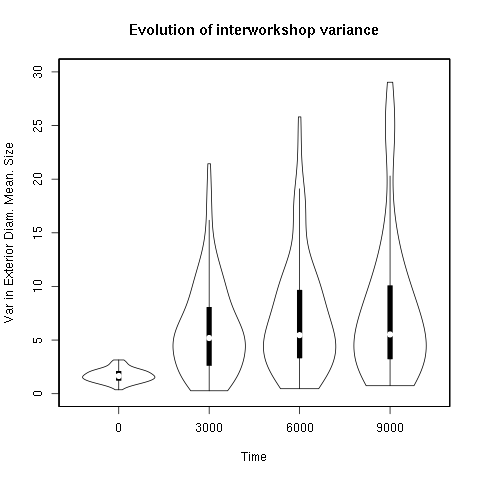
\includegraphics[height=.3\textwidth]{images/cubeC.png}
	    &
	    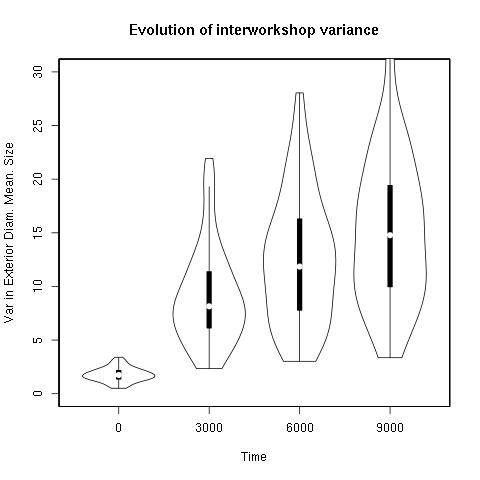
\includegraphics[height=.3\textwidth]{images/lineNC.png}\\
	\end{tabular}
	\label{fig:resmod}
    \end{figure}


    
\end{column}
 % End of the second column
\end{columns}

\end{block}
\end{column}

%BEGIN LAST COLUMN----------------------------------------------------

\begin{column}{\sepwid}\end{column} % Empty spacer column

\begin{column}{\onecolwid} % The third column

\begin{block}{Concluding Remarks}
\justify

Empirical studies identified a variation on the making techniques processes among pottery workshops. We observe that this variability is affected by the distance: amphorae made in nearby workshops with a minor spacial distance share more similar traits than amphorae made in pottery workshops farther. It suggests that the pottery techniques were learned from master to disciple instead of workers with the same level. 

The theoretical model support those claim as it shows that when introducing the possibility of horizontal transmission between the workshop the diversity of production quickly decrease.
 
\end{block}

\begin{block}{References}
\small

\begin{thebibliography}{50}

\bibitem[1]{mesoudi}\textsc{Mesoudi, A. (2015)}
\textit{Cultural Evolution: A review of Theory, Finding and Controversies}, Evolutionary biology.

\bibitem[2]{agui}\textsc{Aguilera, A. (1998)}
\textit{An\'alisis multivariable: una nueva v\'ia para la caracterizaci\'on cer\'amica}, Pyranae, 29.

\bibitem[3]{schillinger}\textsc{Schillinger, K. et al. (2006)}
\textit{Differences in Manufacturing Traditions and Assemblage-Level Patterns: the Origins of Cultural Differences in Archaeological Data}, Journal of Archaeological Method Theory.

\bibitem[4]{li}\textsc{Li, A. (2014)}
\textit{Crossbows and imperial craft organisation: the bronze triggers of China's Terracotta Army}, Antiquity, 88.339.

\end{thebibliography}

\end{block}

%----------------------------------------------------------------------------------------
%	ACKNOWLEDGEMENTS
%----------------------------------------------------------------------------------------

\setbeamercolor{block title}{fg=dblue,bg=white} % Change the block title color

\begin{block}{Acknowledgements}

\small{\rmfamily{The Funding for this work was provided by the ERC Advanced Grant EPNet (340828)}}

\end{block}

%----------------------------------------------------------------------------------------
%	CONTACT INFORMATION
%----------------------------------------------------------------------------------------

\setbeamercolor{block alerted title}{fg=white,bg=dblue!70} % Change the alert block title colors
\setbeamercolor{block alerted body}{fg=black,bg=white} % Change the alert block body colors


\begin{center}
\begin{tabular}{ccc}

\includegraphics[width=0.4\linewidth]{images/epnet.png} & \hfill & 
\includegraphics[width=0.4\linewidth]{images/erc.png}
\end{tabular}
\end{center}

%----------------------------------------------------------------------------------------

\end{column} % End of the third column

\end{columns} % End of all the columns in the poster

\end{frame} % End of the enclosing frame

\end{document}
